\documentclass[10pt,conference]{IEEEtran}
\IEEEoverridecommandlockouts
% The preceding line is only needed to identify funding in the first footnote. If that is unneeded, please comment it out.
\usepackage{cite}
\usepackage{amsmath,amssymb,amsfonts}
\usepackage{algorithmic}
\usepackage{graphicx}
\graphicspath{{figures/}}
\usepackage[spaces,hyphens]{xurl}
\usepackage{textcomp}
\usepackage{xcolor}
\def\BibTeX{{\rm B\kern-.05em{\sc i\kern-.025em b}\kern-.08em
    T\kern-.1667em\lower.7ex\hbox{E}\kern-.125emX}}

\begin{document}

\title{An Exploratory Study of Project Activity Changepoints in Open Source Software Evolution}

\author{\IEEEauthorblockN{James Walden}
\IEEEauthorblockA{\textit{Department of Computer Science} \\
\textit{Northern Kentucky University}\\
Highland Heights, KY USA\\
waldenj@nku.edu}
\and
\IEEEauthorblockN{Noah Burgin}
% \IEEEauthorblockA{\textit{Department of Electrical Engineering\\ and Computer Science} \\
 \IEEEauthorblockA{\textit{Department of EE and Computer Science} \\
    \textit{University of Tennessee}\\
Knoxville, TN USA\\
noah22@vols.utk.edu}
\and
\IEEEauthorblockN{Kuljit Kaur}
\IEEEauthorblockA{\textit{Department of Computer Science} \\
\textit{Guru Nanak Dev University}\\ 
Amritsar, India\\
kuljitchahal.cse@gndu.ac.in} 
}
\maketitle

\begin{abstract}
We used a nonparametric changepoint detection algorithm to measure the smoothness of open source software evolution. Our dataset consisted of 8,919 projects with at least four years of history selected from the World of Code.
We found changepoints in project activity time series in 99\% of the projects, with most projects having between one and six changepoints. Increases and decreases in project activity occur with roughly equal frequency. While most changes are relatively small, on the order of a few authors or few dozen commits per month, there were long tails of much larger project activity changes.
\end{abstract}

\begin{IEEEkeywords}
software evolution, changepoints, world of code
\end{IEEEkeywords}

\section{Introduction}

We performed an exploratory study of changepoints in open source project activity during the MSR 2021 hackathon. We analyzed project activity time series obtained from the World of Code~\cite{ma2019world}, an archive cross-referencing over 120 million git repositories from multiple forges. We selected 8,919 projects from the World of Code that had sufficient historical data to compute monthly time series of project activity.

Lehman's laws of software evolution~\cite{lehman1996laws} describe how time series that describe characteristics of software, such as complexity or functionality, evolve in the long run. However, these laws do not address the question of whether such time series are smooth or punctuated by changepoints. Changepoints are data points in a time series, where the statistical properties of the data points before and after the changepoint differ significantly. 

A five stage model of the software lifecycle has been proposed to explain how project activity changes throughout the lifecycle of a project~\cite{rajlich2000staged}. The model was adapted to account for multiple phases of growth and stabilization found in open source software evolution~\cite{capiluppi2007adapting}. Like many studies of software evolution, these papers analyzed software time series visually for a small number of projects.

% However, changepoint analysis has been used in the software performance literature to identify instances when performance changed significantly~\cite{cito2014identifying,muhlbauer2020identifying}. 
% Two prior case studies of open source projects visually identified changepoints in development activity of a single project~\cite{gonzalez2014studying,openssl2020} without using a changepoint detection algorithm. 

In contrast, we analyzed thousands of projects using a changepoint detection algorithm~\cite{van2020evaluation} to measure the prevalence and size of changepoints in open source software evolution. The two research questions for this exploratory study were:
\begin{enumerate}
    \item How common are changepoints in open source project activity?
    \item What are the sizes and magnitudes of changes at changepoints?
\end{enumerate}

\section{Data}

In order to have a sufficiently quantity of data for changepoint analysis, we selected open source projects that had at a lifespan of at least four years, with at least 50 commit authors and 5000 commits. We found 8,919 projects that met our criteria. We identified projects that met our criteria using the MongoDB \texttt{WoC.proj\_metadata.S} collection. Project selection was completed in a few minutes.

During the course of the multi-week virtual hackathon, World of Code (WoC) data transitioned from version R to version S. We adapted data collection scripts and procedures written for version R to use the new version, in order to gain access to the new \texttt{rootfork} field it provided. Forges like GitHub contain many forks of popular projects, making it difficult to identify the repository that is used by the project team for development. Prior to version S, the only measure of centrality in a cluster of projects was algorithmically determined within WoC. The \texttt{rootfork} field identifies the true root project based on data provided by GitHub.

We collected two monthly time series for each project: number of commits and number of authors that made one or more commits during the month. Time series were computed using the \texttt{getValues} commands that access data in pre-computed maps and tables within WoC. To get all commits for a selected project, we used the \texttt{p2c} map. We then used the \texttt{c2ta} map to retrieve the timestamp and author of each commit. A python script grouped commits by month, counting the number of commits per month and the number of unique authors who made those commits. Running these processes on World of Code servers took four days. As other hackathon projects were simultaneously using these servers, it may be possible to compute the time series in a shorter amount of time.

% Since World of Code does not provide a map from commits to time and files changed, we used WoC's python interface, \texttt{oscar.py} to compute time series for the number of files changed. Commit objects in the python interface provided the needed timestamps and files changed per commit data. Commits were grouped by month and were used to compute the number of files changed per month.

\section{Changepoint analysis}

As our time series data was not normally distributed, we used the nonparametric PELT (Pruned Exact Linear Time) algorithm for changepoint detection. We used the implementation in version 1.0.2 of the R \texttt{changepoint.np} package~\cite{killick2014changepoint}. We used the algorithm's default parameters, with the exception of specifying the minimum segment length to be three months, as we wanted to find changes in activity that were somewhat durable instead of looking for anomalous months. 

% We did not perform hyperparameter optimization, as we did not have a dataset of project activity time series with labeled changepoints to evaluate algorithm performance. An evaluation of multiple changepoint algorithms on a variety of time series~\cite{van2020evaluation} from different fields of study found little improvement from hyperparameter optimization of this algorithm in any case.

We found that more than 99\% of projects have changepoints in project activity. Only 55 projects had no changepoints in their author time series, and the median number of changepoints was three. Most projects (94\%) had between one and six changepoints. There are outliers, with six projects having 10 changepoints and one project having 14 changepoints. No project had between 11 and 13 changepoints. We can see the distribution of projects by number of changepoints in Figure~\ref{fig:authorcpts}.
\begin{figure}[ht!]
    \centering
    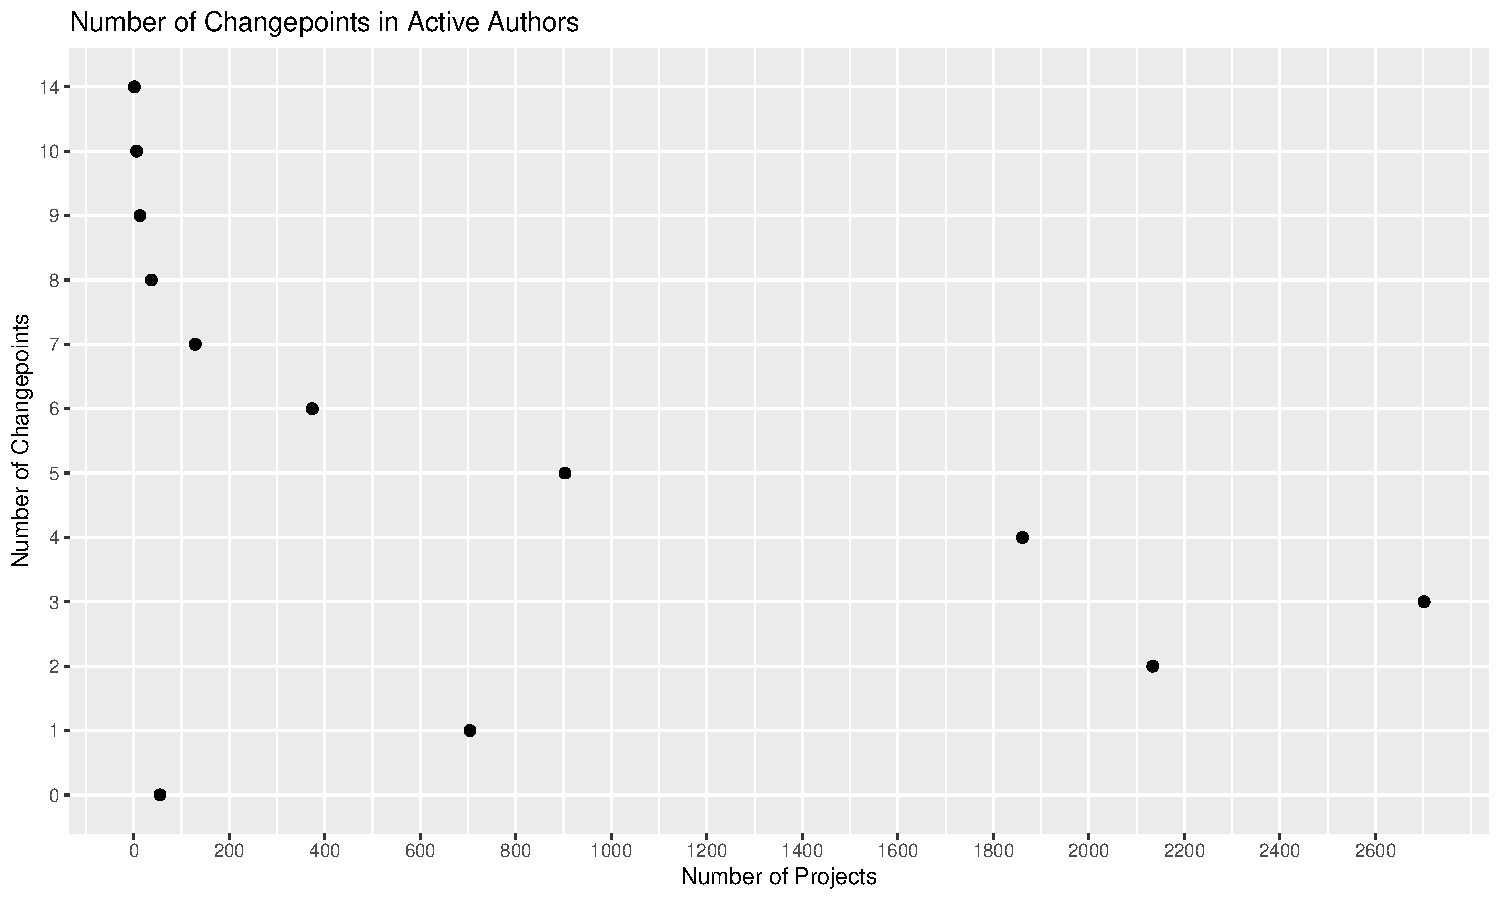
\includegraphics[width=\linewidth]{author-changepoints.pdf}
    \caption{Number of Changepoints in Author Time Series}
    \label{fig:authorcpts}
\end{figure}

The median number of changepoints in the commits per month time series was also three, with 32 projects having no changepoints. Most projects (90\%) had between one and six changepoints. Outliers consisted of 27 projects with ten or more changepoints, including a single project with 16 changepoints.
\begin{figure}[ht!]
    \centering
    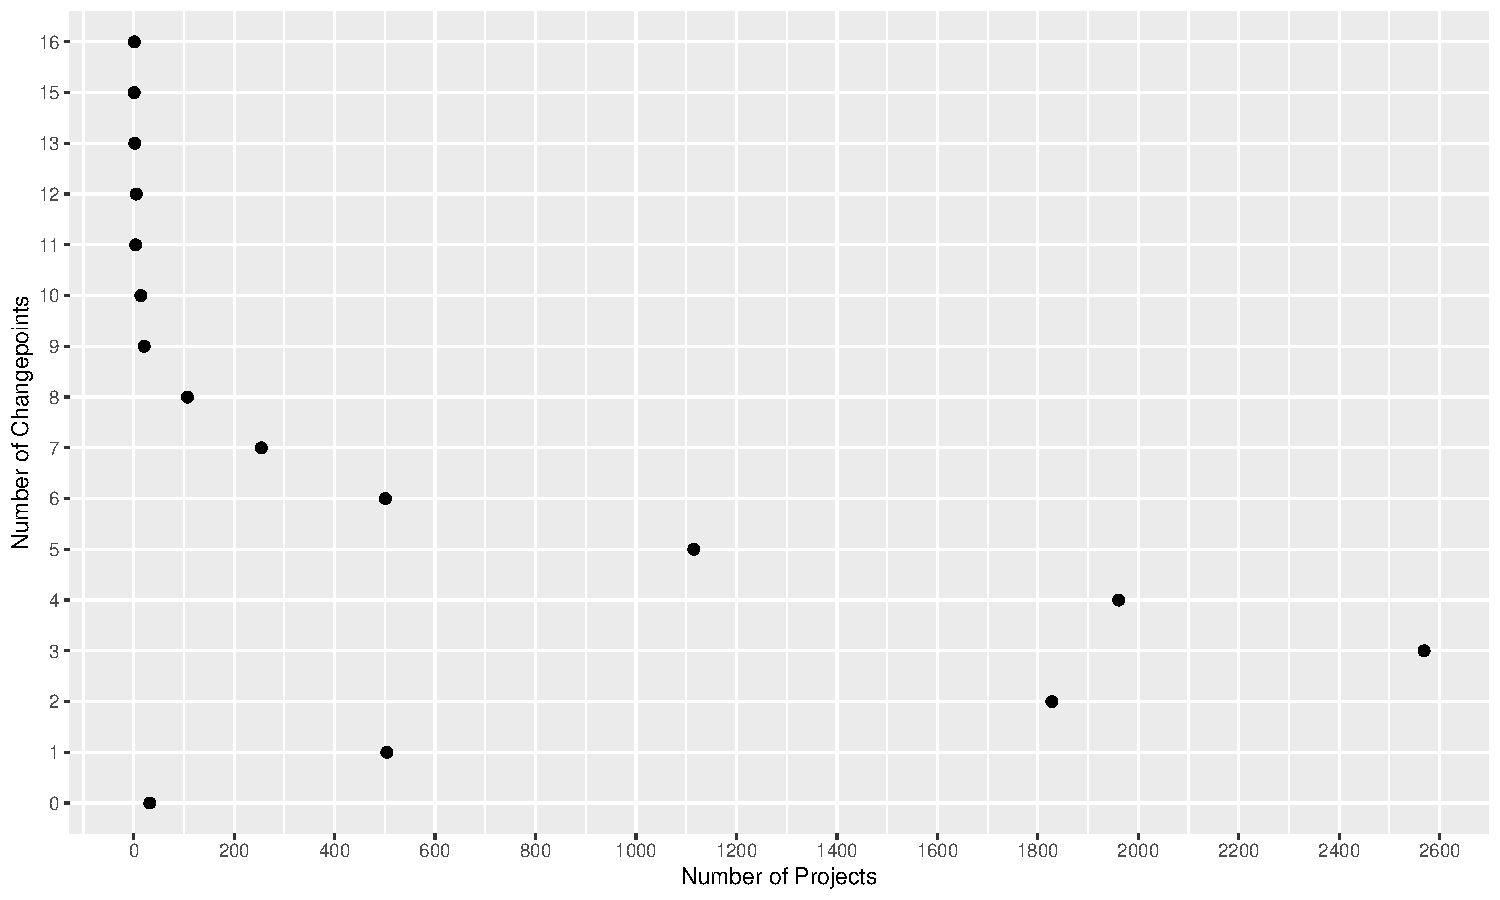
\includegraphics[width=\linewidth]{commit-changepoints.pdf}
    \caption{Number of Changepoints in Commit Time Series}
    \label{fig:commitcpts}
\end{figure}

We found a total of 31,416 changepoints in project commit time series, of which 15,342 (49\%) were increases in commit activity and 16,047 (51\%) were reductions in activity. We computed the magnitude of a changepoint as the difference in means in the number of monthly commits before and after the changepoint. The size of most changes were relatively small, with the interquartile range (IQR) ranging between -75 to 87 commits per month, but there was a substantial tail in both directions as can be seen in Figure~\ref{fig:commitsizes}.
\begin{figure}[ht!]
    \centering
    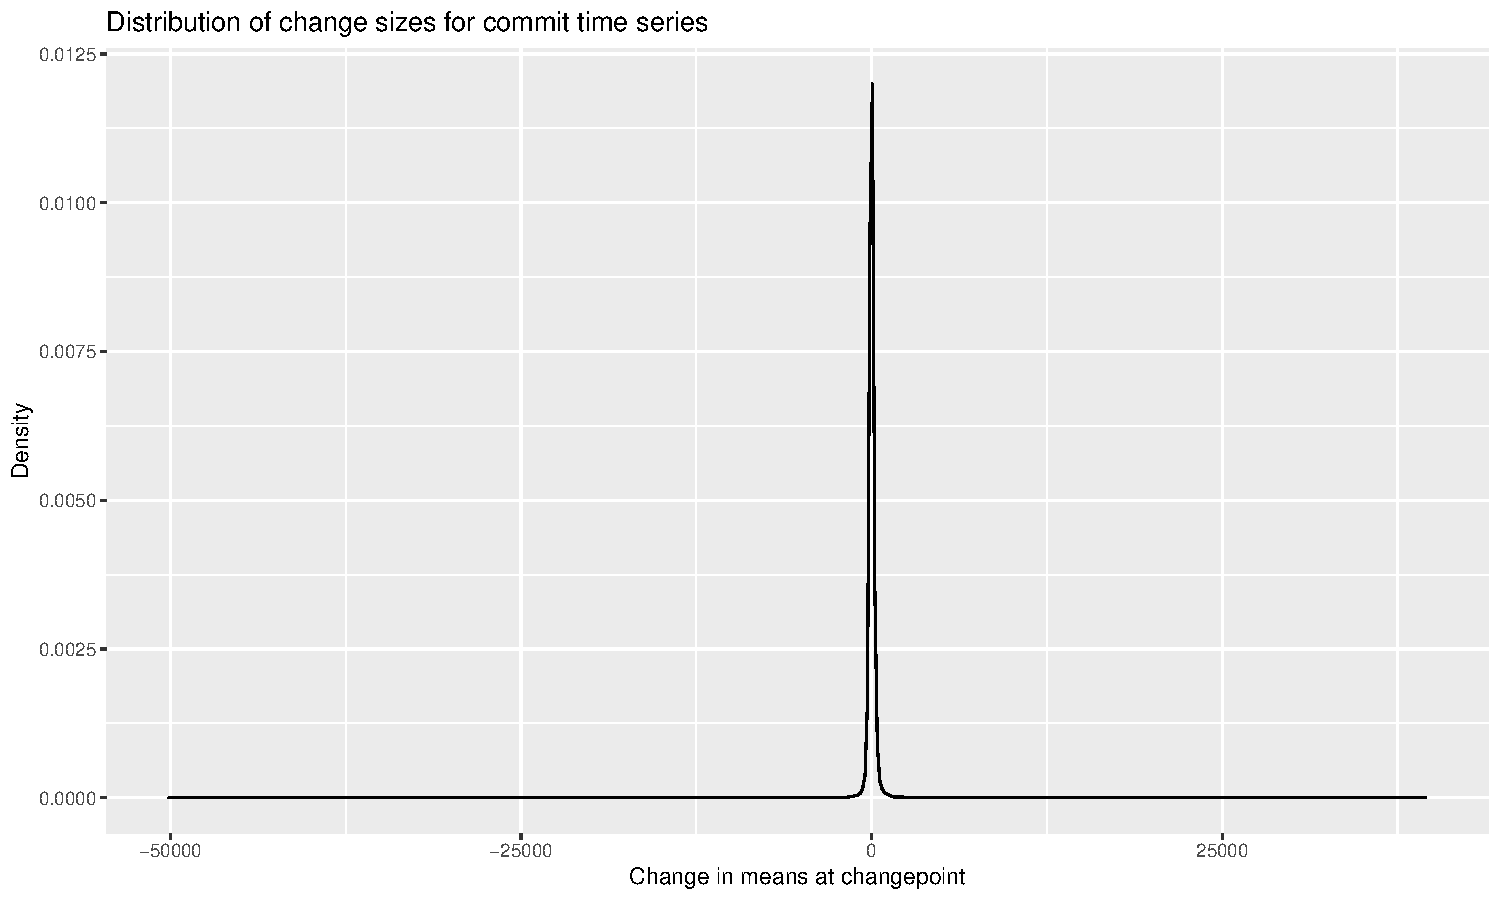
\includegraphics[width=\linewidth]{commit-changesizes.pdf}
    \caption{Size of Changes in Commit Time Series}
    \label{fig:commitsizes}
\end{figure}

Our results for the signs and magnitude of author time series changes were similar. We found 28,671 changepoints in author time series, of which 12,114 (42\%) were reductions in activity and 16,557 (58\%) were increases in activity. Changes in the number of contributing authors per month were relatively small, with IQR ranging between -3.4 to 5.8 authors per month, but there was a substantial tail in both directions. The graph for author time series is identical in appearance to Figure~\ref{fig:commitsizes} but with smaller values on the x-axis.
% as can be seen in Figure~\ref{fig:authorsizes}.
% \begin{figure}[ht!]
%     \centering
%     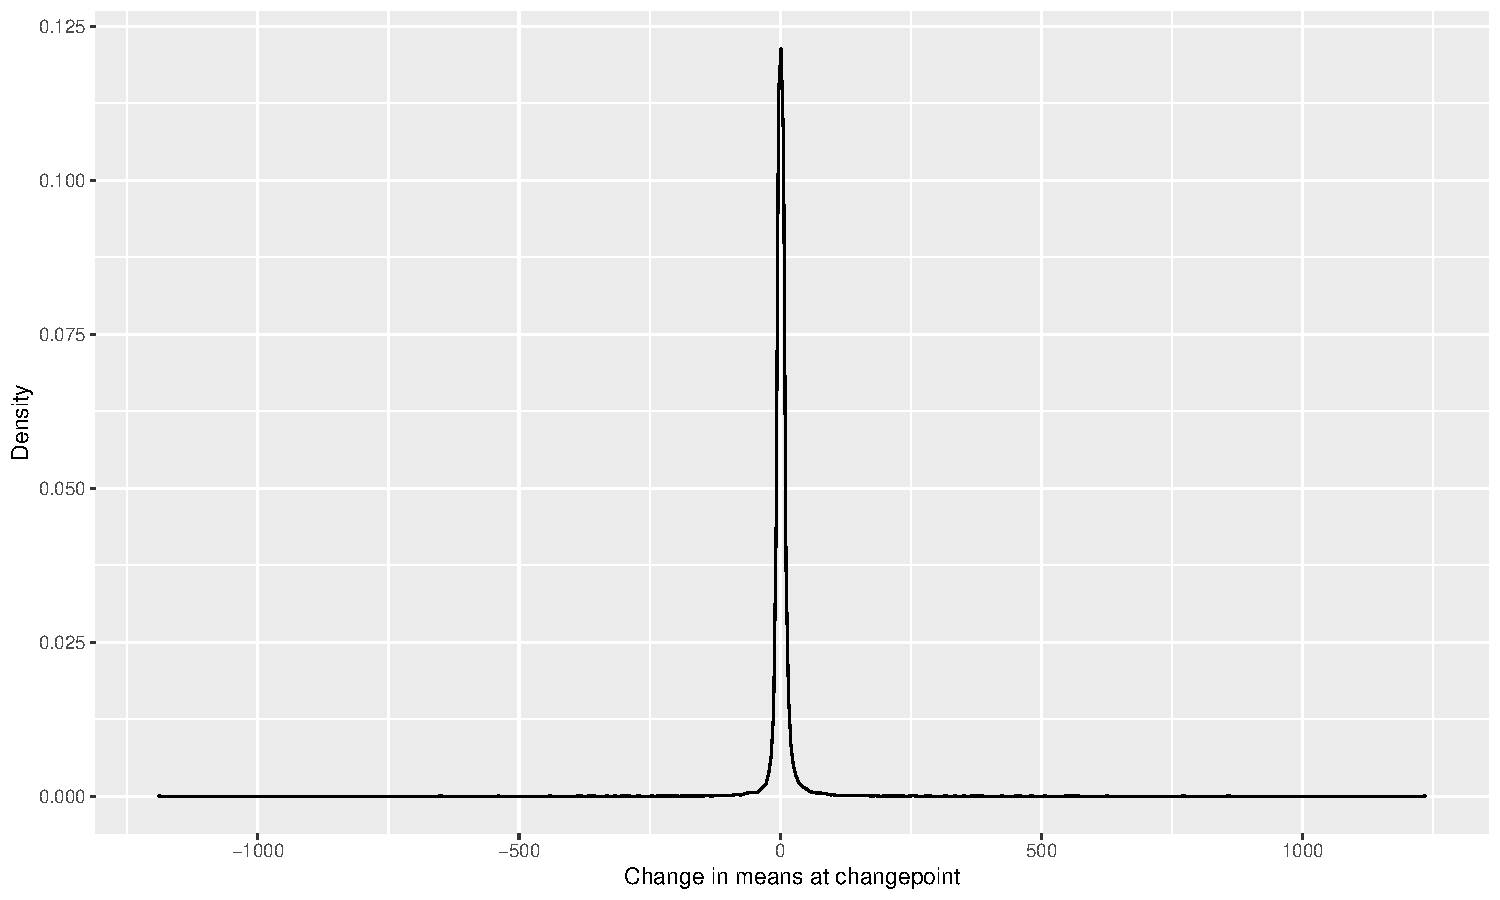
\includegraphics[width=\linewidth]{author-changesizes.pdf}
%     \caption{Size of Changes in Author Time Series}
%     \label{fig:commitsizes}
% \end{figure}

\section{Conclusion}

We found that open source evolution is rarely smooth and typically includes changepoints, points where the size and/or direction of evolution changes significantly. The vast majority of projects have between one and six changepoints in both the number of monthly commits and number of unique authors per month, while some outliers have up to 16 changepoints. Changepoints that decrease or increase project activity occur with roughly equal frequency. While most changepoints are relatively small (a few authors per month, a few dozen commits per month), there is a long tail of much larger changes. The data and code used in this project can be found in the project's git repository at \url{https://github.com/woc-hack/inflection-points}.

In the future, we plan to study patterns of changepoints and to examine changepoints in software characteristics beyond project activity. Patterns may point towards a common software lifecycle model or common responses to external events, such as security incidents~\cite{openssl2020}. We also plan to investigate the causes of changepoints, with a focus on the long tail of large changes. We would also like to explore software evolution more broadly. Large open source projects, like the Linux kernel, often use multiple repositories. World of Code provides information about clusters of repositories, which we could use to investigate patterns of software evolution in such projects.

\bibliographystyle{IEEEtran}
\bibliography{changepoints-msr2021}

\end{document}
